\documentclass[a4paper,11pt]{article}
\usepackage{a4wide}
\usepackage{fullpage}
\usepackage[utf8x]{inputenc}

\usepackage[light,math]{anttor}
\usepackage[T1]{fontenc}

%\usepackage[slovene]{babel}
%\selectlanguage{slovene}
\usepackage[toc,page]{appendix}
\usepackage[pdftex]{graphicx} 

\usepackage{lmodern}
\usepackage{amsmath}
\usepackage{amssymb}
\usepackage{amsthm}
\usepackage{amsfonts}
\usepackage{mathtools}
\usepackage{enumitem}
\usepackage{amsfonts}
\usepackage{amsmath}
\usepackage{setspace}
\usepackage{color}
\definecolor{light-gray}{gray}{0.95}
\usepackage{listings} 
\usepackage{hyperref}

\renewcommand{\baselinestretch}{1.2} 
\renewcommand{\appendixpagename}{Priloge}


\title{Algoritmi \\
\textbf{Domača naloga 1} }
\author{Sara Bizjak}
\date{Marec 2021}

%%%%%%%%%%%%%%%%%%%%%%%%%%%%%%%%%%%%%%%%%%%%%%%%%%%%%%%%%%%%%%%%%%%%%%%%%%%%%%%%%%%%%%%%%%%%%%%%%%%%%%%%%%%%%%%%%%%%%%%%%%%%%%%%%

\begin{document}

\maketitle

%%%%%%%%%%%%%%%%%%%%%%%%%%%%%%%%%%%%%%%%%%%%%%%%%%%%%%%%%%%%%%%%%%%%%%%%%%%%%%%%%%%%%%

\section*{Problem 1 -- Turingov stroj}

Sestavimo TS za množenje dveh števil, ki sta na traku podani v eniškem zapisu. 
\\
Poglejmo si primer množenja števil 3 in 4, kot je podan v navodilih naloge. 
Trak \textit{inputa} v tem primeru bi izgledal 
$$
B \ B \ 1 \ 1 \ 1 \ 0 \ 1 \ 1 \ 1 \ 1 \ 0 \ B \ B \ B \ B \ B \ \ldots
$$
kjer prve tri enke predstavljajo število 3, druge štiri pa število 4.
Ideja je, da za vsako enko izmed prvih treh, druge štiri enke kopiramo naprej na trak, kjer so sedaj zapisani $B$-ji oziroma prazni prostori.
Rezultat tega kopiranja bodo tako $3 \cdot 4 = 12$ enke, kar je ravno rezultat množenja med tema dvema številoma.
$$
B \ B \ B \ B \ B \ B \ B \ B \ B \ B \ B \ 1 \ 1 \ 1 \ 1 \ 1 \ 1 \ 1 \ 1 \ 1 \ 1 \ 1 \ 1 \ 0 \ B \ B \ B \ \ldots
$$
\noindent
Turingov stroj je bil konstruiran in testiran s pomočjo spletne strani \cite{bib:TS}.
Koda za poganjanje TS-ja na tej strani:

\begin{lstlisting}
________________________________________________________________________
//-------CONFIGURATION
name: TS za mnozenje dveh enisko podanih stevil
init: q0
accept: q8

//-------DELTA FUNCTION:
q0,1
q1,_,>

q1,1
q1,1,>

q1,0
q2,0,>

q2,1
q3,Y,>

q3,1
q3,1,>

q3,0
q3,0,>

q3,_
q4,1,<

q4,1
q4,1,<

q4,0
q4,0,<

q4,Y
q2,Y,>

q2,0
q5,0,<

q5,Y
q5,1,<

q5,0
q5,0,<

q5,1
q5,1,<

q5,_
q0,_,>

q0,0
q6,_,>

q6,1
q6,_,>

q6,0
q7,_,>

q7,1
q7,1,>

q7,_
q8,0,>
________________________________________________________________________

\end{lstlisting}

\noindent
Pripadajoč tranzicijski graf:
\begin{figure}[ht!]
    \centering
    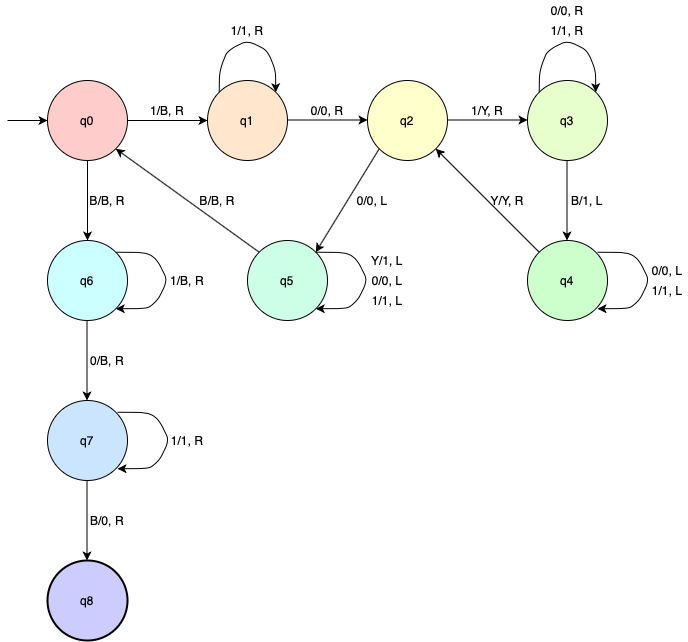
\includegraphics[width=150mm]{graf.png}
    \caption{Graf tranzicij stanj TS za množenje dveh eniško podanih števil.}
\end{figure}

\section*{Problem 2 -- Prevedba}
Pokažimo, da je problem delitve (\textit{partition problem}) NP-poln s prevedbo na problem seštevka podmnožic (\textit{subset-sum}). 
Cilj problema delitve je, da multi-množico pozitivnih celih števil $S$ razdelimo na dve podmnožici tako, da bosta vsoti elementov enaki.
Označimo ti dve podmnožici s $S_1$ in $S_2 = S - S_1$, kjer je $N_1$ vsota elementov iz $S_1$, $N_2$ pa vsota elementov iz $S_2$, tako da
$$
\sum_{s \ \in \ S_1} s = \sum_{s \ \in \ S_2} s 
$$
$$
\Rightarrow N_1 = N_2
$$
Ker je NP-poln problem hkrati NP in NP-težek problem, je za NP-polnost problema $L$ potrebno dokazati dvoje:
\begin{enumerate}
    \item Problem $L$ je \textbf{vsebovan v razredu NP}.
    \item Vsak drug (znan) problem $L'$ iz razreda NP lahko v polinomskem času prevedemo na problem $L$. 
\end{enumerate}
\noindent
Če problem ustreza drugemu pogoju, pravimo, da je problem NP-težek.
\\
\\
\textit{Dokažimo najprej vsebovanost problema v razredu NP.}
\\
Za primer delitve so cetrifikati množica $S$ in particiji $S_1$ in $S_2$. 
Očitno je, da lahko vsote obeh podmnožic preverimo v polinomskem (linearnem) času po naslednjem postopku:
\begin{enumerate}
    \item Preverimo, da z elementi iz $S_1$ in $S_2$ pokrijemo celoten $S$.
    \item Nastavimo $N_1 = 0$ in $N_2 = 0$.
    \item Za vsak element $s$ iz $S_1$ prištejemo njegovo vrednost $N_1$.
    \item Za vsak element $s$ iz $S_2$ prištejemo njegovo vrednost $N_2$.
    \item Preverimo, da sta vrednost $N_1$ in $N_2$ enaki.
\end{enumerate}
Ker lahko problem delitve rešimo v polinomskem času na nedetetminističnem TS, je torej vsebovan v razredu NP problemov.
\\
\\
\textit{Dokažimo še, da je problem delitve NP-težek.}
\\
Da bi pokazali, da je problem delitve NP-težek, reduciramo nek znan NP-poln problem, v našem primeru je to problem seštevka podmnožic, na problem delitve.
Pri reševanju problema seštevka podmnožic za \textit{input} vzamemo množico pozitivnih celih števil $S$ in končno, ciljno vsoto $t$. 
Poiskati moramo podmnožico $T \subset S$, katere vsota elementov je enaka $t$. 
Označimo z $N$ vsoto elementov iz $S$, torej $\sum_{s \in S} s = N$ in definirajmo množico 
$$S' = S \cup \{ N - 2t \},$$ 
ki jo podamo v problem delitve. 
Ta redukcija očitno deluje v polinomskem času.
Pokažimo sedaj, da taka redukcija res obstaja. 
\\
Denimo, da je $T$ množica števil z vsoto enako $t$. Tedaj imajo preostali elementi iz $S$, to množico označimo s $S_{rest}$, vsoto $N_{rest} = N - t$. 
Nadalje, naj bo množica $T' = T \cup \{ N - 2t \}$ z vsoto $t'$.
\\
Tedaj velja:
\begin{align*}
    N_{rest}  &= N - t 
    \\
    N_{rest}  - t &= N - 2t, 
\end{align*}
\noindent
kar nam podaja razliko med množicama $S_{rest}$ in množico $T$.
\\
Nadalje velja::
\begin{align*}
    t' &= t + (N - 2t) 
\\
    &= s - t 
\\
    &= N_{rest},
\end{align*}
\noindent
kar pomeni, da sta vsoti elementov množic $T'$ in $S_{rest}$ enaki.
\\
Začetno množico $S$ lahko torej razdelimo na dve podmnožici, označili smo jih s $T'$ in s $S_{rest}$, katerih vsota elementov je pri obeh podmnožicah enaka $(N - t)$. 
\\
\\
S tem smo dokazali NP-polnost problema delitve.

\section*{Problem 3 -- Rodovne funkcije}
Izračunajmo na koliko načinov lahko dobimo vsoto $500 {}{∏ÍÔÓÌ}

%%%%%%%%%%%%%%%%%%%%%%%%%%%%%%%%%%%%%%%%%%%%%%%%%%%%%%%%%%%%%%%%%%%%%%%%%%%%%%%%%%%%%%
\begin{thebibliography}{99}
    \bibitem{bib:TS}
    Platforma za vizualizacijo in testiranje TS, dostopna na \url{https://turingmachinesimulator.com}.
\end{thebibliography}

\end{document}